\newif\ifteacher\teachertrue
\documentclass[11pt,a4paper]{article}
\usepackage[margin=2.4cm,top=2.2cm]{geometry}
\usepackage{amsmath,amssymb}
\usepackage{tgschola}\usepackage{fouriernc}
\linespread{1.05}
\usepackage[T1]{fontenc}
\usepackage{microtype}
\usepackage{tikz}
\usetikzlibrary{angles,quotes,calc,arrows.meta}
\usepackage{enumitem}
\usepackage{needspace}
\usepackage{tfrupee}
\definecolor{figline}{RGB}{64,64,64}
\definecolor{figfill}{RGB}{232,232,232}
\definecolor{figfill2}{RGB}{214,214,214}
\definecolor{muted}{RGB}{72,74,78}
\definecolor{thinrule}{RGB}{128,128,128}
\pagestyle{plain}
\setlength{\parindent}{0pt}
\setlength{\parskip}{1pt}
\setlength{\lineskiplimit}{2pt}\setlength{\lineskip}{4pt}
\setlength{\emergencystretch}{2em}
\tikzset{fig/.style={draw=figline}}
\newcommand{\nl}{\\[3pt]}
\newcounter{qn}
\newcommand{\ques}{\par\medskip\refstepcounter{qn}\noindent\hangindent=1.7em\hangafter=1\makebox[1.7em][l]{\textbf{\arabic{qn}.}}\ignorespaces}
\newcommand{\pc}[2]{\par\smallskip\noindent\hspace*{2em}\hangindent=4.3em\hangafter=1\makebox[2em][l]{(#1)}\hspace{0.3em}#2\par}
\newcommand{\mcqone}[4]{\par\smallskip\noindent\hspace*{2em}\hangindent=4.3em\hangafter=1(a)~#1 \qquad (b)~#2 \qquad (c)~#3 \qquad (d)~#4\par}
\newcommand{\mcqtwo}[4]{\par\smallskip\noindent\hspace*{2em}\begin{tabular}[t]{@{}p{0.42\linewidth}@{\hspace{1.6em}}p{0.42\linewidth}@{}}(a)~#1 & (b)~#2 \\[5pt](c)~#3 & (d)~#4\end{tabular}\par\smallskip}
\newcommand{\optline}[1]{\par\vspace{2pt}\noindent\hspace*{2em}\hangindent=4.3em\hangafter=1 #1}
\newcommand{\aritem}[2]{\par\smallskip\noindent\hspace*{1.7em}\hangindent=1.7em\hangafter=1 #1:~#2\par}
\newcommand{\orline}{\par\smallskip{\centering\textit{OR}\par}\nopagebreak\smallskip}
\newcommand{\sect}[1]{\par\medskip\Needspace{15\baselineskip}{\small\bfseries #1}\par\nopagebreak\smallskip}
\ifteacher
\newenvironment{answerblock}
  {\par\needspace{6\baselineskip}\smallskip\begingroup\small\linespread{1.2}\selectfont\color{muted}\noindent\textit{Solution.}\par}
  {\par\endgroup\medskip}
\newcommand{\ap}[1]{\par\smallskip\noindent\textbf{(#1)}\ }
\else
\usepackage{comment}
\excludecomment{answerblock}
\fi
\makeatletter
\newcommand{\figslot}[1]{\@ifundefined{fig@#1}{}{\csname fig@#1\endcsname}}
\makeatother
\newcommand{\mks}[1]{\hfill\mbox{[#1]}}
\newcommand{\tr}{\triangle}
\newcommand{\Given}{\textbf{Given:}~}
\newcommand{\Tofind}{\textbf{To find:}~}
\newcommand{\Toprove}{\textbf{To prove:}~}
\newcommand{\Constr}{\textbf{Construction:}~}
\newcommand{\Ans}{\textbf{Answer:}~}
\newcommand{\Hp}{Hence proved.}
\begin{document}
\begin{center}
{\Large\bfseries Circles}\\[3pt]
{\large\bfseries Test 1}\\[5pt]
Date: \rule{3cm}{0.4pt} \quad Duration: 1 hour 30 minutes \quad Maximum marks: 40
\end{center}
\vspace{-6pt}
\noindent\rule{\linewidth}{0.6pt}\par
\vspace{3pt}
{\centering\small All questions are compulsory. Draw a rough diagram wherever it helps. Show all your steps and give reasons.\par}
\ifteacher
\vspace{4pt}
{\color{thinrule}\noindent\rule{\linewidth}{0.4pt}}\par
\vspace{4pt}
{\small\color{muted}\linespread{1.15}\selectfont
\textbf{Paper design.} The paper follows the CBSE pattern. Section A: $6\times1$ mark (4 multiple-choice questions, 1 fill-in-the-blank question and 1 assertion--reason question). Section B: $4\times2$ marks. Section C: $4\times3$ marks. Section D: $2\times5$ marks. Section E: 1 case-based question of 4 marks. Total: 40 marks.\nl
\textbf{Theorem numbers.} The paper uses the theorem numbers of the class notes (Circles classes 1--4). Theorems 1--4 carry about 27 marks. Theorems 5--8 carry about 13 marks. Theorems 9--12 are not assessed.\nl
\textbf{Competency focus.} Question 2 tests direct use of a result. The other questions are competency-based. Students find an error (Q7), work backwards (Q10, Q16), write proofs (Q12, Q15), construct a figure (Q13), compare chords (Q5, Q14) and apply results to real situations (Q8, Q13, Q16, Q17).\nl
\textbf{Concepts assessed.} Equal chords and angles at the centre, Theorems 1 and 2 (Q1, 8, 12, 17); the line from the centre to a chord, Theorems 3 and 4 (Q2, 3, 6, 7, 9, 10, 11, 14, 15, 16, 17); the circle through three points, Theorem 5 (Q4, 13); chords and their distance from the centre, Theorems 6--8 (Q5, 9, 14, 16, 17).\nl
\textbf{Common misconceptions.} Joining the centre to any point of a chord and taking the line as perpendicular (Q7); using the full chord in place of half the chord in Pythagoras theorem (Q2, 10, 11); adding the distances in every case of parallel chords (Q11).\nl
\textbf{Marking.} Award method marks for a correct set-up, even where the final computation contains an arithmetic error. In proofs, award marks for the correct congruence rule with all three conditions and their reasons.\par}
\vspace{4pt}
{\color{thinrule}\noindent\rule{\linewidth}{0.4pt}}\par
\vspace{3pt}
\fi
\sect{Section A (1 mark each)}
{\small\itshape Questions 1, 2, 3 and 5 are multiple choice. Question 4 is fill in the blank. Question 6 is assertion--reason.\par}

\Needspace{8\baselineskip}
\ques In a circle with centre $O$, chords $AB$ and $CD$ are equal and $\angle OAB=55^\circ$. What is $\angle COD$? \mks{1}
\mcqtwo{$55^\circ$}{$70^\circ$}{$110^\circ$}{$125^\circ$}
\begin{answerblock}
\begin{minipage}[t]{0.66\linewidth}\vspace{0pt}
\Ans (b) $70^\circ$.
\begin{enumerate}[label=\arabic*.,leftmargin=1.6em,itemsep=0pt,topsep=2pt]
\item $OA=OB$ (radii), so $\angle OBA=\angle OAB=55^\circ$.
\item $\angle AOB=180^\circ-55^\circ-55^\circ=70^\circ$ (angle sum of a triangle).
\item $\angle COD=\angle AOB=70^\circ$ (equal chords subtend equal angles at the centre, Theorem 1).
\end{enumerate}
\end{minipage}\hfill
\begin{minipage}[t]{0.3\linewidth}\vspace{0pt}
\centering
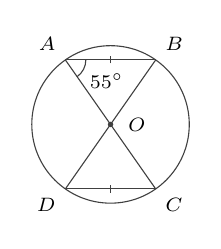
\begin{tikzpicture}[fig,every node/.style={font=\scriptsize}]
\draw (0,0) circle (1);
\coordinate (O) at (0,0);
\coordinate (A) at (-0.5736,0.8192);
\coordinate (B) at (0.5736,0.8192);
\coordinate (C) at (0.5736,-0.8192);
\coordinate (D) at (-0.5736,-0.8192);
\draw (A)--(B);
\draw (C)--(D);
\draw (O)--(A);
\draw (O)--(B);
\draw (O)--(C);
\draw (O)--(D);
\draw (A) ++(0:0.26) arc[start angle=0,end angle=-55,radius=0.26];
\node at (-0.05,0.55) {$55^\circ$};
\draw (0,0.775)--(0,0.865);
\draw (0,-0.865)--(0,-0.775);
\fill[figline] (O) circle (0.035);
\node[above left] at (A) {$A$};
\node[above right] at (B) {$B$};
\node[below right] at (C) {$C$};
\node[below left] at (D) {$D$};
\node[right] at (0.1,0) {$O$};
\end{tikzpicture}
\end{minipage}
\end{answerblock}

\Needspace{8\baselineskip}
\ques A chord of length $20$~cm is drawn in a circle of radius $26$~cm. What is the distance of the chord from the centre? \mks{1}
\mcqtwo{$6$~cm}{$16$~cm}{$24$~cm}{$28$~cm}
\begin{answerblock}
\begin{minipage}[t]{0.66\linewidth}\vspace{0pt}
\Ans (c) $24$~cm.
\begin{enumerate}[label=\arabic*.,leftmargin=1.6em,itemsep=0pt,topsep=2pt]
\item $OM\perp AB$, so $AM=10$~cm (the perpendicular from the centre bisects the chord, Theorem 4).
\item $OM^2=26^2-10^2=676-100=576$, so $OM=24$~cm (Pythagoras theorem).
\end{enumerate}
\end{minipage}\hfill
\begin{minipage}[t]{0.3\linewidth}\vspace{0pt}
\centering
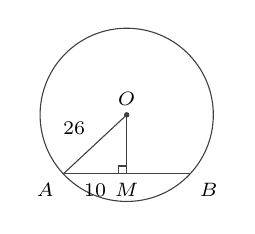
\begin{tikzpicture}[fig,every node/.style={font=\scriptsize}]
\coordinate (O) at (0,0); \coordinate (A) at (-0.805,-0.75); \coordinate (B) at (0.805,-0.75); \coordinate (M) at (0,-0.75);
\draw (O) circle (1.1); \draw (A)--(B); \draw (O)--(A); \draw (O)--(M);
\draw (M) ++(-0.1,0) -- ++(0,0.1) -- ++(0.1,0);
\fill[figline] (O) circle (0.035);
\node[above] at (O) {$O$}; \node[below left] at (A) {$A$}; \node[below right] at (B) {$B$}; \node[below] at (M) {$M$};
\node[above left] at ($(O)!0.5!(A)$) {$26$}; \node[below] at ($(A)!0.5!(M)$) {$10$};
\end{tikzpicture}
\end{minipage}
\end{answerblock}

\Needspace{8\baselineskip}
\ques Which statement about a circle with centre $O$ is \textbf{false}? \mks{1}
\pc{a}{The line joining $O$ to the midpoint of a chord (not a diameter) is perpendicular to the chord.}
\pc{b}{The perpendicular from $O$ to a chord bisects the chord.}
\pc{c}{The perpendicular bisector of every chord passes through $O$.}
\pc{d}{Every line through $O$ bisects every chord of the circle.}
\begin{answerblock}
\begin{minipage}[t]{0.66\linewidth}\vspace{0pt}
\Ans (d). A line through $O$ that is slanted to a chord (not a diameter) meets the chord away from its midpoint. Statements (a), (b) and (c) are Theorems 3 and 4 and their consequence.
\end{minipage}\hfill
\begin{minipage}[t]{0.3\linewidth}\vspace{0pt}
\centering
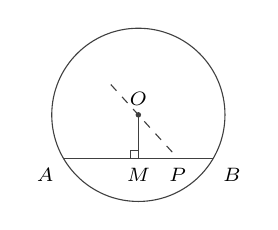
\begin{tikzpicture}[fig,every node/.style={font=\scriptsize}]
\coordinate (O) at (0,0); \coordinate (A) at (-0.953,-0.55); \coordinate (B) at (0.953,-0.55); \coordinate (M) at (0,-0.55); \coordinate (P) at (0.5,-0.55);
\draw (O) circle (1.1); \draw (A)--(B); \draw (O)--(M);
\draw (M) ++(-0.1,0) -- ++(0,0.1) -- ++(0.1,0);
\draw[dashed] ($(O)!-0.7!(P)$) -- (P);
\fill[figline] (O) circle (0.035);
\node[above] at (O) {$O$}; \node[below left] at (A) {$A$}; \node[below right] at (B) {$B$}; \node[below] at (M) {$M$}; \node[below] at (P) {$P$};
\end{tikzpicture}
\end{minipage}
\end{answerblock}

\Needspace{8\baselineskip}
\ques Fill in the blank: The number of circles that pass through three points lying on one straight line is \rule{1.5cm}{0.4pt}. \mks{1}
\begin{answerblock}
\begin{minipage}[t]{0.66\linewidth}\vspace{0pt}
\Ans $0$ (none). The perpendicular bisectors of $AB$ and $BC$ are parallel, so they never meet. No point is at the same distance from all three points. (Theorem 5 needs three non-collinear points.)
\end{minipage}\hfill
\begin{minipage}[t]{0.3\linewidth}\vspace{0pt}
\centering
\begin{tikzpicture}[fig,every node/.style={font=\scriptsize}]
\draw (-0.4,0) -- (2.4,0);
\foreach \x/\l in {0/A,0.8/B,2.0/C} {\fill[figline] (\x,0) circle (0.035); \node[below] at (\x,-0.05) {$\l$};}
\draw[dashed] (0.4,-0.55) -- (0.4,0.7); \draw[dashed] (1.4,-0.55) -- (1.4,0.7);
\end{tikzpicture}
\end{minipage}
\end{answerblock}

\Needspace{8\baselineskip}
\ques A circle has radius $10$~cm. It has two chords of lengths $12$~cm and $18$~cm. Which chord is nearer the centre? \mks{1}
\mcqtwo{The $12$~cm chord}{The $18$~cm chord}{Both are at the same distance}{It cannot be decided without more information}
\begin{answerblock}
\begin{minipage}[t]{0.66\linewidth}\vspace{0pt}
\Ans (b). Of two chords of a circle, the longer chord is nearer the centre (Theorem 8).
\end{minipage}\hfill
\begin{minipage}[t]{0.3\linewidth}\vspace{0pt}
\centering
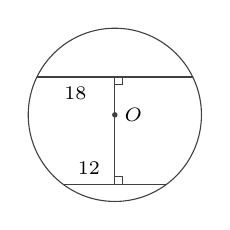
\begin{tikzpicture}[fig,every node/.style={font=\scriptsize}]
\coordinate (O) at (0,0);
\draw (O) circle (1.1);
\draw (-0.99,0.48) -- (0.99,0.48); \draw (-0.66,-0.88) -- (0.66,-0.88);
\draw (O) -- (0,0.48); \draw (O) -- (0,-0.88);
\draw (0,0.48) ++(0.1,0) -- ++(0,-0.1) -- ++(-0.1,0);
\draw (0,-0.88) ++(0.1,0) -- ++(0,0.1) -- ++(-0.1,0);
\fill[figline] (O) circle (0.035);
\node[right] at (O) {$O$};
\node[below] at (-0.5,0.48) {$18$}; \node[above] at (-0.33,-0.88) {$12$};
\end{tikzpicture}
\end{minipage}
\end{answerblock}

\Needspace{8\baselineskip}
\ques Assertion--reason. {\small\itshape Choose: (a) Both A and R are true, and R is the correct explanation of A. (b) Both A and R are true, but R is not the correct explanation of A. (c) A is true, but R is false. (d) A is false, but R is true.\par}
\aritem{Assertion (A)}{In a circle with centre $O$, $OM\perp AB$, where $AB$ is a chord and $M$ lies on $AB$. If $AM=5$~cm, then $AB=10$~cm.}
\aritem{Reason (R)}{The perpendicular from the centre of a circle to a chord bisects the chord. \mks{1}}
\begin{answerblock}
\begin{minipage}[t]{0.66\linewidth}\vspace{0pt}
\Ans (a). $OM\perp AB$, so $M$ is the midpoint of $AB$ (Theorem 4). So $AB=2\times5=10$~cm. R is the reason for A.
\end{minipage}\hfill
\begin{minipage}[t]{0.3\linewidth}\vspace{0pt}
\centering
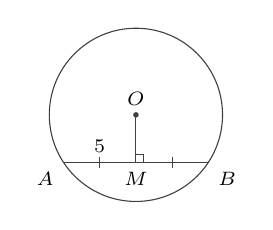
\begin{tikzpicture}[fig,every node/.style={font=\scriptsize}]
\coordinate (O) at (0,0); \coordinate (A) at (-0.922,-0.6); \coordinate (B) at (0.922,-0.6); \coordinate (M) at (0,-0.6);
\draw (O) circle (1.1); \draw (A)--(B); \draw (O)--(M);
\draw (M) ++(0.1,0) -- ++(0,0.1) -- ++(-0.1,0);
\draw (-0.46,-0.53) -- (-0.46,-0.67); \draw (0.46,-0.53) -- (0.46,-0.67);
\fill[figline] (O) circle (0.035);
\node[above] at (O) {$O$}; \node[below left] at (A) {$A$}; \node[below right] at (B) {$B$}; \node[below] at (M) {$M$};
\node[above] at (-0.46,-0.6) {$5$};
\end{tikzpicture}
\end{minipage}
\end{answerblock}

\sect{Section B (2 marks each)}

\Needspace{8\baselineskip}
\ques In a circle with centre $O$, chord $AB=10$~cm. $P$ is a point on $AB$ with $AP=4$~cm. Meena writes: ``$OP$ is perpendicular to $AB$, because the line joining the centre to a point of a chord is perpendicular to the chord.''
\pc{a}{What is wrong in Meena's reasoning?\mks{1}}
\pc{b}{Which point $Q$ of $AB$ must be joined to $O$ so that $OQ\perp AB$? How far is $Q$ from $A$?\mks{1}}
\begin{answerblock}
\begin{minipage}[t]{0.66\linewidth}\vspace{0pt}
\textbf{(a)} Theorem 3 is true only for the line from the centre to the \emph{midpoint} of the chord. $P$ is not the midpoint: $AP=4$~cm but $PB=6$~cm. So $OP$ is not perpendicular to $AB$.

\textbf{(b)} $Q$ is the midpoint of $AB$ (Theorem 3), so $AQ=\dfrac{10}{2}=5$~cm.

\Ans $Q$ is the midpoint of $AB$; $AQ=5$~cm.
\end{minipage}\hfill
\begin{minipage}[t]{0.3\linewidth}\vspace{0pt}
\centering
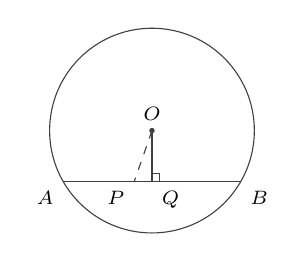
\begin{tikzpicture}[fig,every node/.style={font=\scriptsize}]
\coordinate (O) at (0,0); \coordinate (A) at (-1.126,-0.65); \coordinate (B) at (1.126,-0.65); \coordinate (Q) at (0,-0.65); \coordinate (P) at (-0.226,-0.65);
\draw (O) circle (1.3); \draw (A)--(B); \draw (O)--(Q); \draw[dashed] (O)--(P);
\draw (Q) ++(0.1,0) -- ++(0,0.1) -- ++(-0.1,0);
\fill[figline] (O) circle (0.035);
\node[above] at (O) {$O$}; \node[below left] at (A) {$A$}; \node[below right] at (B) {$B$};
\node[below left] at (P) {$P$}; \node[below right] at (Q) {$Q$};
\end{tikzpicture}
\end{minipage}
\end{answerblock}

\Needspace{8\baselineskip}
\ques Divya draws a circle with centre $O$ for a rangoli. She marks $10$ dots on the circle at equal distances and numbers them $1$ to $10$ in order. She joins dot $1$ to dot $4$, and dot $6$ to dot $9$ with straight lines.
\begin{center}
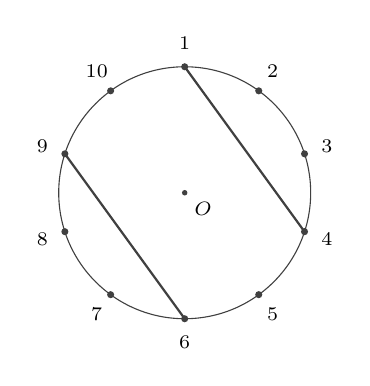
\begin{tikzpicture}[fig,every node/.style={font=\scriptsize}]
\draw (0,0) circle (1.6);
\fill[figline] (0,0) circle (0.035);
\node[below right] at (0,0) {$O$};
\fill[figline] (0,1.6) circle (0.045);
\fill[figline] (0.9405,1.2944) circle (0.045);
\fill[figline] (1.5217,0.4944) circle (0.045);
\fill[figline] (1.5217,-0.4944) circle (0.045);
\fill[figline] (0.9405,-1.2944) circle (0.045);
\fill[figline] (0,-1.6) circle (0.045);
\fill[figline] (-0.9405,-1.2944) circle (0.045);
\fill[figline] (-1.5217,-0.4944) circle (0.045);
\fill[figline] (-1.5217,0.4944) circle (0.045);
\fill[figline] (-0.9405,1.2944) circle (0.045);
\draw[thick] (0,1.6)--(1.5217,-0.4944);
\draw[thick] (0,-1.6)--(-1.5217,0.4944);
\node at (0,1.9) {$1$};
\node at (1.1168,1.5371) {$2$};
\node at (1.8070,0.5871) {$3$};
\node at (1.8070,-0.5871) {$4$};
\node at (1.1168,-1.5371) {$5$};
\node at (0,-1.9) {$6$};
\node at (-1.1168,-1.5371) {$7$};
\node at (-1.8070,-0.5871) {$8$};
\node at (-1.8070,0.5871) {$9$};
\node at (-1.1168,1.5371) {$10$};
\end{tikzpicture}
\end{center}
\pc{a}{Find the angle that the line from dot $1$ to dot $4$ subtends at $O$.\mks{1}}
\pc{b}{Show that the two lines are equal in length.\mks{1}}
\begin{answerblock}
\begin{minipage}[t]{0.66\linewidth}\vspace{0pt}
\Given $10$ equally spaced dots on a circle with centre $O$; chords from dot $1$ to dot $4$ and from dot $6$ to dot $9$.

\Tofind (a) the angle at $O$; (b) show the chords are equal.

\begin{enumerate}[label=\arabic*.,leftmargin=1.6em,itemsep=0pt,topsep=2pt]
\item The $10$ dots divide the full angle $360^\circ$ at $O$ into $10$ equal angles of $\dfrac{360^\circ}{10}=36^\circ$.
\item From dot $1$ to dot $4$ there are $3$ gaps, so the angle is $3\times36^\circ=108^\circ$.
\item From dot $6$ to dot $9$ there are also $3$ gaps, so that angle is also $108^\circ$.
\item The two chords subtend equal angles at the centre, so they are equal (Theorem 2).
\end{enumerate}
\Ans (a) $108^\circ$; (b) the chords are equal.
\end{minipage}\hfill
\begin{minipage}[t]{0.3\linewidth}\vspace{0pt}
\centering
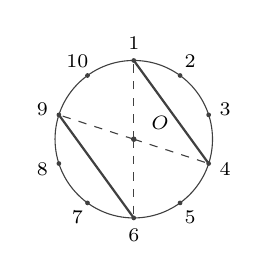
\begin{tikzpicture}[fig,every node/.style={font=\scriptsize}]
\coordinate (O) at (0,0);
\draw (O) circle (1);
\foreach \k in {1,...,10} {\fill[figline] ({90-36*(\k-1)}:1) circle (0.03); \node at ({90-36*(\k-1)}:1.22) {\k};}
\draw[thick] (90:1) -- (-18:1); \draw[thick] (-90:1) -- (162:1);
\draw[dashed] (O) -- (90:1); \draw[dashed] (O) -- (-18:1); \draw[dashed] (O) -- (-90:1); \draw[dashed] (O) -- (162:1);
\fill[figline] (O) circle (0.035);
\node[anchor=south west] at (0.1,0.0) {$O$};
\end{tikzpicture}
\end{minipage}
\end{answerblock}

\Needspace{8\baselineskip}
\ques Chords $PQ$ and $RS$ of a circle with centre $O$ are each $16$~cm from $O$, and $PQ=24$~cm.
\pc{a}{Find $RS$. Give the reason.\mks{1}}
\pc{b}{Find the radius of the circle.\mks{1}}
\begin{answerblock}
\begin{minipage}[t]{0.66\linewidth}\vspace{0pt}
\Given $OM\perp PQ$, $ON\perp RS$, $OM=ON=16$~cm, $PQ=24$~cm.

\Tofind $RS$ and the radius.

\begin{enumerate}[label=\arabic*.,leftmargin=1.6em,itemsep=0pt,topsep=2pt]
\item $PQ$ and $RS$ are equidistant from $O$, so $RS=PQ=24$~cm (Theorem 7).
\item $PM=\dfrac{24}{2}=12$~cm (Theorem 4).
\item $OP^2=OM^2+PM^2=256+144=400$, so $OP=20$~cm (Pythagoras theorem).
\end{enumerate}
\Ans $RS=24$~cm; radius $20$~cm.
\end{minipage}\hfill
\begin{minipage}[t]{0.3\linewidth}\vspace{0pt}
\centering
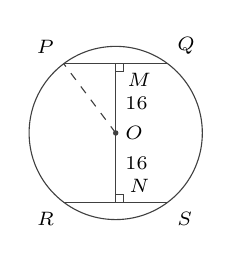
\begin{tikzpicture}[fig,every node/.style={font=\scriptsize}]
\coordinate (O) at (0,0); \coordinate (M) at (0,0.88); \coordinate (N) at (0,-0.88);
\draw (O) circle (1.1);
\draw (-0.66,0.88) -- (0.66,0.88); \draw (-0.66,-0.88) -- (0.66,-0.88);
\draw (O)--(M); \draw (O)--(N); \draw[dashed] (O) -- (-0.66,0.88);
\draw (M) ++(0.1,0) -- ++(0,-0.1) -- ++(-0.1,0);
\draw (N) ++(0.1,0) -- ++(0,0.1) -- ++(-0.1,0);
\fill[figline] (O) circle (0.035);
\node[right] at (O) {$O$};
\node[above left] at (-0.66,0.88) {$P$}; \node[above right] at (0.66,0.88) {$Q$};
\node[below left] at (-0.66,-0.88) {$R$}; \node[below right] at (0.66,-0.88) {$S$};
\node[below] at (0.3,0.88) {$M$}; \node[above] at (0.3,-0.88) {$N$};
\node[right] at (0,0.38) {$16$}; \node[right] at (0,-0.38) {$16$};
\end{tikzpicture}
\end{minipage}
\end{answerblock}

\Needspace{8\baselineskip}
\ques A chord of a circle is $18$~cm long and is $12$~cm from the centre. Find the diameter of the circle. Draw a rough diagram that shows the circle, its centre $O$, the chord $AB$ and the perpendicular $OM$ from $O$ to $AB$. Mark the given lengths on it. \mks{2}
\begin{answerblock}
\begin{minipage}[t]{0.66\linewidth}\vspace{0pt}
\Given chord $AB=18$~cm, $OM\perp AB$, $OM=12$~cm.

\Tofind the diameter.

\begin{enumerate}[label=\arabic*.,leftmargin=1.6em,itemsep=0pt,topsep=2pt]
\item $AM=\dfrac{18}{2}=9$~cm (Theorem 4).
\item $OA^2=OM^2+AM^2=144+81=225$, so $OA=15$~cm (Pythagoras theorem).
\item Diameter $=2\times15=30$~cm.
\end{enumerate}
\Ans $30$~cm.
\end{minipage}\hfill
\begin{minipage}[t]{0.3\linewidth}\vspace{0pt}
\centering
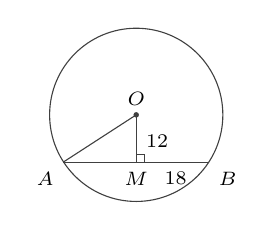
\begin{tikzpicture}[fig,every node/.style={font=\scriptsize}]
\coordinate (O) at (0,0); \coordinate (A) at (-0.926,-0.6); \coordinate (B) at (0.926,-0.6); \coordinate (M) at (0,-0.6);
\draw (O) circle (1.1); \draw (A)--(B); \draw (O)--(M); \draw (O)--(A);
\draw (M) ++(0.1,0) -- ++(0,0.1) -- ++(-0.1,0);
\fill[figline] (O) circle (0.035);
\node[above] at (O) {$O$}; \node[below left] at (A) {$A$}; \node[below right] at (B) {$B$}; \node[below] at (M) {$M$};
\node[right] at (0,-0.33) {$12$}; \node[below] at (0.5,-0.6) {$18$};
\end{tikzpicture}
\end{minipage}
\end{answerblock}
\setcounter{qn}{10}
\sect{Section C (3 marks each)}

\Needspace{8\baselineskip}
\ques $AB$ and $CD$ are parallel chords of a circle with centre $O$ and radius $25$~cm. $AB=40$~cm and $CD=30$~cm.
\pc{a}{Find the distance of each chord from $O$.\mks{1}}
\pc{b}{Find the distance between the chords when they lie on the same side of $O$.\mks{1}}
\pc{c}{Find the distance between the chords when they lie on opposite sides of $O$.\mks{1}}

For (b) and (c), draw a rough diagram of each case. Show the circle, its centre $O$, both chords, and one line through $O$ perpendicular to both chords.

\begin{answerblock}
\begin{minipage}[t]{0.60\linewidth}\vspace{0pt}
\Given radius $25$~cm, $AB\parallel CD$, $AB=40$~cm, $CD=30$~cm; $OM\perp AB$, $ON\perp CD$. \Tofind $OM$, $ON$ and the distance $MN$ in both cases.
\begin{enumerate}[label=\arabic*.,leftmargin=1.6em,itemsep=0pt,topsep=2pt]
\item $AM=20$~cm and $CN=15$~cm (Theorem 4).
\item $OM^2=25^2-20^2=625-400=225$, so $OM=15$~cm (Pythagoras theorem).
\item $ON^2=25^2-15^2=625-225=400$, so $ON=20$~cm.
\item $M$, $O$, $N$ lie on one line perpendicular to both chords. Same side: $MN=ON-OM=20-15=5$~cm.
\item Opposite sides: $MN=OM+ON=15+20=35$~cm.
\end{enumerate}
\Ans (a) $AB$ is $15$~cm and $CD$ is $20$~cm from $O$; (b) $5$~cm; (c) $35$~cm.
\end{minipage}\hfill
\begin{minipage}[t]{0.38\linewidth}\vspace{0pt}
\centering
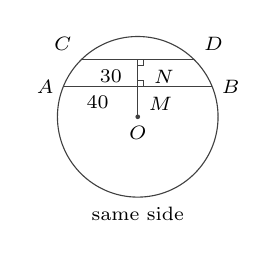
\begin{tikzpicture}[fig,scale=0.85,every node/.style={font=\scriptsize}]
\coordinate (O) at (0,0);
\draw (O) circle (1.2);
\draw (-1.112,0.45) -- (1.112,0.45); \draw (-0.847,0.85) -- (0.847,0.85);
\draw (O) -- (0,0.85);
\draw (0,0.45) ++(0.09,0) -- ++(0,0.09) -- ++(-0.09,0);
\draw (0,0.85) ++(0.09,0) -- ++(0,-0.09) -- ++(-0.09,0);
\fill[figline] (O) circle (0.035);
\node[below] at (O) {$O$};
\node[left] at (-1.112,0.45) {$A$}; \node[right] at (1.112,0.45) {$B$};
\node[above left] at (-0.847,0.85) {$C$}; \node[above right] at (0.847,0.85) {$D$};
\node[anchor=north west] at (0.02,0.44) {$M$}; \node[anchor=north west] at (0.1,0.84) {$N$};
\node[below] at (-0.6,0.45) {$40$}; \node[below] at (-0.4,0.85) {$30$};
\node at (0,-1.45) {same side};
\end{tikzpicture}\hfill
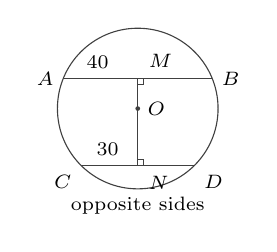
\begin{tikzpicture}[fig,scale=0.85,every node/.style={font=\scriptsize}]
\coordinate (O) at (0,0);
\draw (O) circle (1.2);
\draw (-1.112,0.45) -- (1.112,0.45); \draw (-0.847,-0.85) -- (0.847,-0.85);
\draw (0,0.45) -- (0,-0.85);
\draw (0,0.45) ++(0.09,0) -- ++(0,-0.09) -- ++(-0.09,0);
\draw (0,-0.85) ++(0.09,0) -- ++(0,0.09) -- ++(-0.09,0);
\fill[figline] (O) circle (0.035);
\node[right] at (O) {$O$};
\node[left] at (-1.112,0.45) {$A$}; \node[right] at (1.112,0.45) {$B$};
\node[below left] at (-0.847,-0.85) {$C$}; \node[below right] at (0.847,-0.85) {$D$};
\node[anchor=south west] at (0.02,0.46) {$M$}; \node[anchor=north west] at (0.02,-0.86) {$N$};
\node[above] at (-0.6,0.45) {$40$}; \node[above] at (-0.45,-0.85) {$30$};
\node at (0,-1.45) {opposite sides};
\end{tikzpicture}
\end{minipage}
\end{answerblock}

\Needspace{8\baselineskip}
\ques $AB$ and $CD$ are equal chords of a circle with centre $O$. Prove that $\angle OAB=\angle OCD$. \mks{3}

\begin{center}
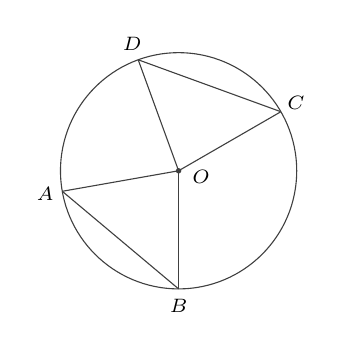
\begin{tikzpicture}[fig,every node/.style={font=\scriptsize}]
\coordinate (O) at (0,0); \coordinate (A) at (190:1.5); \coordinate (B) at (270:1.5); \coordinate (C) at (30:1.5); \coordinate (D) at (110:1.5);
\draw (O) circle (1.5);
\draw (A)--(B); \draw (C)--(D);
\draw (O)--(A); \draw (O)--(B); \draw (O)--(C); \draw (O)--(D);
\fill[figline] (O) circle (0.035);
\node[right] at (0.05,-0.08) {$O$};
\node at (190:1.72) {$A$}; \node at (270:1.72) {$B$}; \node at (30:1.72) {$C$}; \node at (110:1.72) {$D$};
\end{tikzpicture}
\end{center}

\begin{answerblock}
\begin{minipage}[t]{0.66\linewidth}\vspace{0pt}
\Given $AB$ and $CD$ are chords of a circle with centre $O$, $AB=CD$. \Toprove $\angle OAB=\angle OCD$. \Constr join $OA$, $OB$, $OC$, $OD$. Proof: In $\tr OAB$ and $\tr OCD$:
\begin{enumerate}[label=\arabic*.,leftmargin=1.6em,itemsep=0pt,topsep=2pt]
\item $OA=OC$ (radii).
\item $OB=OD$ (radii).
\item $AB=CD$ (given).
\item So $\tr OAB\cong\tr OCD$ (SSS rule).
\item So $\angle OAB=\angle OCD$ (corresponding parts of congruent triangles).
\end{enumerate}
\Hp
\end{minipage}\hfill
\begin{minipage}[t]{0.3\linewidth}\vspace{0pt}
\centering
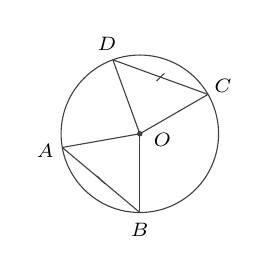
\begin{tikzpicture}[fig,every node/.style={font=\scriptsize}]
\coordinate (O) at (0,0); \coordinate (A) at (190:1.0); \coordinate (B) at (270:1.0); \coordinate (C) at (30:1.0); \coordinate (D) at (110:1.0);
\draw (O) circle (1.0);
\draw (A)--(B); \draw (C)--(D);
\draw (O)--(A); \draw (O)--(B); \draw (O)--(C); \draw (O)--(D);
\fill[figline] (O) circle (0.035);
\node[right] at (0.05,-0.08) {$O$};
\node at (190:1.22) {$A$}; \node at (270:1.22) {$B$}; \node at (30:1.22) {$C$}; \node at (110:1.22) {$D$};
\draw ($(A)!0.5!(B)+(-0.05,0.05)$) -- ($(A)!0.5!(B)+(0.05,-0.05)$);
\draw ($(C)!0.5!(D)+(-0.05,-0.05)$) -- ($(C)!0.5!(D)+(0.05,0.05)$);
\end{tikzpicture}
\end{minipage}
\end{answerblock}

\Needspace{8\baselineskip}
\ques Three houses $A$, $B$ and $C$ stand in a village. $AB=300$~m, $BC=400$~m and $\angle ABC=90^\circ$. The panchayat wants to dig a well at a point $W$ that is at the same distance from all three houses.
\pc{a}{Use the scale $1$~cm $=50$~m. Draw $AB=6$~cm. At $B$, draw $\angle ABC=90^\circ$ and mark $C$ with $BC=8$~cm. Join $AC$.\mks{1}}
\pc{b}{Construct the perpendicular bisectors of $AB$ and $BC$. Mark their meeting point $W$.\mks{1}}
\pc{c}{Measure $WA$. Find the real distance of the well from each house.\mks{1}}

\begin{answerblock}
\begin{minipage}[t]{0.66\linewidth}\vspace{0pt}
\Given $AB=300$~m, $BC=400$~m, $\angle B=90^\circ$; scale $1$~cm $=50$~m. \Tofind the position of $W$ and its distance from each house.
\begin{enumerate}[label=\arabic*.,leftmargin=1.6em,itemsep=0pt,topsep=2pt]
\item $AB=\dfrac{300}{50}=6$~cm and $BC=\dfrac{400}{50}=8$~cm on paper.
\item Every point on the perpendicular bisector of $AB$ is equally far from $A$ and $B$; every point on the perpendicular bisector of $BC$ is equally far from $B$ and $C$. So $W$ is equally far from $A$, $B$ and $C$. It is the centre of the only circle through $A$, $B$ and $C$ (Theorem 5).
\item $W$ falls on $AC$, at its midpoint. $AC^2=6^2+8^2=100$, so $AC=10$~cm and $WA=5$~cm (check by measuring).
\item Real distance $=5\times50=250$~m.
\end{enumerate}
\Ans the well is $250$~m from each house.
\end{minipage}\hfill
\begin{minipage}[t]{0.3\linewidth}\vspace{0pt}
\centering
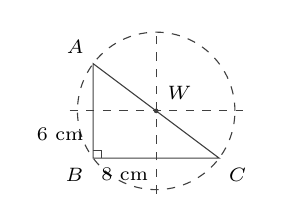
\begin{tikzpicture}[fig,every node/.style={font=\scriptsize}]
\coordinate (B) at (0,0); \coordinate (A) at (0,1.2); \coordinate (C) at (1.6,0); \coordinate (W) at (0.8,0.6);
\draw[dashed] (W) circle (1.0);
\draw (A)--(B)--(C)--cycle;
\draw (B) ++(0.1,0) -- ++(0,0.1) -- ++(-0.1,0);
\draw[dashed] (-0.3,0.6) -- (1.9,0.6); \draw[dashed] (0.8,-0.45) -- (0.8,1.65);
\fill[figline] (W) circle (0.03);
\node[above left] at (A) {$A$}; \node[below left] at (B) {$B$}; \node[below right] at (C) {$C$};
\node[anchor=south west] at (0.82,0.62) {$W$};
\node[left] at (0,0.3) {$6$ cm}; \node[below] at (0.4,0) {$8$ cm};
\end{tikzpicture}
\end{minipage}
\end{answerblock}

\Needspace{8\baselineskip}
\ques A circle has centre $O$ and radius $30$~cm. Chord $AB=48$~cm and chord $CD=36$~cm.
\pc{a}{Without calculating, say which chord is nearer the centre. Give the reason.\mks{1}}
\pc{b}{Find the distance of each chord from $O$, and check your answer to (a).\mks{2}}

\begin{answerblock}
\begin{minipage}[t]{0.66\linewidth}\vspace{0pt}
\Given radius $30$~cm, $AB=48$~cm, $CD=36$~cm; $OM\perp AB$, $ON\perp CD$. \Tofind which chord is nearer $O$; $OM$ and $ON$.
\begin{enumerate}[label=\arabic*.,leftmargin=1.6em,itemsep=0pt,topsep=2pt]
\item $AB>CD$, so $AB$ is nearer the centre (Theorem 8).
\item $AM=24$~cm (Theorem 4); $OM^2=900-576=324$, so $OM=18$~cm.
\item $CN=18$~cm (Theorem 4); $ON^2=900-324=576$, so $ON=24$~cm.
\item $18<24$, so $AB$ is nearer. This agrees with (a).
\end{enumerate}
\Ans $AB$ is nearer; $OM=18$~cm, $ON=24$~cm.
\end{minipage}\hfill
\begin{minipage}[t]{0.3\linewidth}\vspace{0pt}
\centering
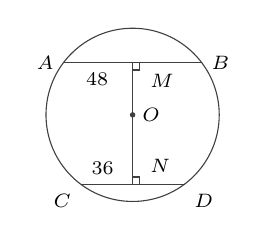
\begin{tikzpicture}[fig,every node/.style={font=\scriptsize}]
\coordinate (O) at (0,0);
\draw (O) circle (1.1);
\draw (-0.88,0.66) -- (0.88,0.66); \draw (-0.66,-0.88) -- (0.66,-0.88);
\draw (0,0.66) -- (0,-0.88);
\draw (0,0.66) ++(0.09,0) -- ++(0,-0.09) -- ++(-0.09,0);
\draw (0,-0.88) ++(0.09,0) -- ++(0,0.09) -- ++(-0.09,0);
\fill[figline] (O) circle (0.035);
\node[right] at (O) {$O$};
\node[left] at (-0.88,0.66) {$A$}; \node[right] at (0.88,0.66) {$B$};
\node[below left] at (-0.66,-0.88) {$C$}; \node[below right] at (0.66,-0.88) {$D$};
\node[anchor=north west] at (0.1,0.64) {$M$}; \node[anchor=south west] at (0.1,-0.86) {$N$};
\node[below] at (-0.45,0.66) {$48$}; \node[above] at (-0.38,-0.88) {$36$};
\end{tikzpicture}
\end{minipage}
\end{answerblock}

\sect{Section D (5 marks each)}

\Needspace{8\baselineskip}
\ques
\pc{a}{Prove that the perpendicular from the centre of a circle to a chord bisects the chord.\mks{3}}
\pc{b}{Two circles have the same centre $O$. A straight line meets the bigger circle at $A$ and $D$, and the smaller circle at $B$ and $C$, in the order $A$, $B$, $C$, $D$ (see the figure). Prove that $AB=CD$.\mks{2}}

\begin{center}
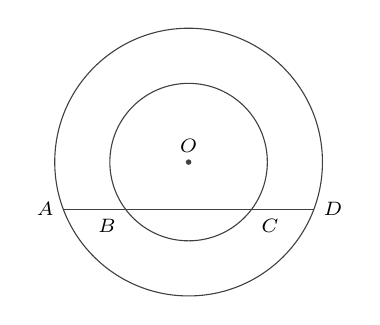
\begin{tikzpicture}[fig,every node/.style={font=\scriptsize}]
\coordinate (O) at (0,0);
\draw (O) circle (1.7); \draw (O) circle (1.0);
\draw (-1.591,-0.6) -- (1.591,-0.6);
\fill[figline] (O) circle (0.035);
\node[above] at (O) {$O$};
\node[left] at (-1.591,-0.6) {$A$}; \node[below left] at (-0.8,-0.6) {$B$};
\node[below right] at (0.8,-0.6) {$C$}; \node[right] at (1.591,-0.6) {$D$};
\end{tikzpicture}
\end{center}

\begin{answerblock}
\textbf{(a)}\\[2pt]
\begin{minipage}[t]{0.66\linewidth}\vspace{0pt}
\Given a circle with centre $O$, chord $AB$, $OM\perp AB$. \Toprove $AM=MB$. \Constr join $OA$ and $OB$. Proof: In $\tr OMA$ and $\tr OMB$:
\begin{enumerate}[label=\arabic*.,leftmargin=1.6em,itemsep=0pt,topsep=2pt]
\item $\angle OMA=\angle OMB=90^\circ$ (given).
\item $OA=OB$ (radii; hypotenuses).
\item $OM=OM$ (common side).
\item So $\tr OMA\cong\tr OMB$ (RHS rule).
\item So $AM=MB$ (corresponding parts of congruent triangles).
\end{enumerate}
\Hp
\end{minipage}\hfill
\begin{minipage}[t]{0.3\linewidth}\vspace{0pt}
\centering
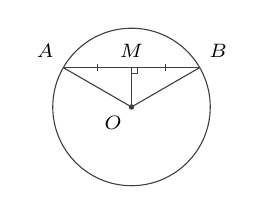
\begin{tikzpicture}[fig,every node/.style={font=\scriptsize}]
\coordinate (O) at (0,0);
\coordinate (A) at (-0.8660,0.5);
\coordinate (B) at (0.8660,0.5);
\coordinate (M) at (0,0.5);
\draw[fig] (O) circle (1);
\draw[fig] (A)--(B);
\draw[fig] (O)--(A);
\draw[fig] (O)--(B);
\draw[fig] (O)--(M);
\fill[figline] (O) circle (0.035);
\draw[fig] (0,0.5)--(0.08,0.5)--(0.08,0.42)--(0,0.42);
\draw[fig] (-0.433,0.455)--(-0.433,0.545);
\draw[fig] (0.433,0.455)--(0.433,0.545);
\node[above left] at (A) {$A$};
\node[above right] at (B) {$B$};
\node[above] at (M) {$M$};
\node[below left] at (O) {$O$};
\end{tikzpicture}
\end{minipage}

\medskip
\textbf{(b)}\\[2pt]
\begin{minipage}[t]{0.66\linewidth}\vspace{0pt}
\Given two circles with centre $O$; a line meets them at $A$, $B$, $C$, $D$ in this order. \Toprove $AB=CD$. \Constr draw $OM\perp AD$. Proof:
\begin{enumerate}[label=\arabic*.,leftmargin=1.6em,itemsep=0pt,topsep=2pt]
\item $AD$ is a chord of the bigger circle, so $AM=MD$ (Theorem 4).
\item $BC$ is a chord of the smaller circle, so $BM=MC$ (Theorem 4).
\item $AB=AM-BM$ and $CD=MD-MC$.
\item So $AB=CD$ (equals subtracted from equals).
\end{enumerate}
\Hp
\end{minipage}\hfill
\begin{minipage}[t]{0.3\linewidth}\vspace{0pt}
\centering
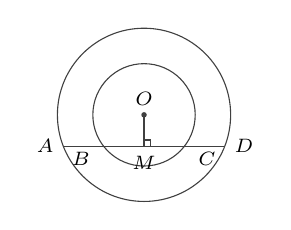
\begin{tikzpicture}[fig,every node/.style={font=\scriptsize}]
\coordinate (O) at (0,0); \coordinate (M) at (0,-0.4);
\draw (O) circle (1.1); \draw (O) circle (0.65);
\draw (-1.025,-0.4) -- (1.025,-0.4); \draw (O)--(M);
\draw (M) ++(0.08,0) -- ++(0,0.08) -- ++(-0.08,0);
\fill[figline] (O) circle (0.035);
\node[above] at (O) {$O$}; \node[below] at (M) {$M$};
\node[left] at (-1.025,-0.4) {$A$}; \node at (-0.8,-0.56) {$B$};
\node at (0.8,-0.56) {$C$}; \node[right] at (1.025,-0.4) {$D$};
\end{tikzpicture}
\end{minipage}
\end{answerblock}

\Needspace{8\baselineskip}
\ques The front of a temple gate has an arch. The arch is part of a circle with centre $O$. The ends $A$ and $B$ of the arch are $16$~m apart. The highest point $T$ of the arch is directly above the midpoint $M$ of $AB$, and $TM=4$~m.

\begin{center}
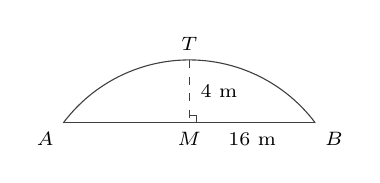
\begin{tikzpicture}[fig,every node/.style={font=\scriptsize}]
\coordinate (A) at (-1.6,1.2); \coordinate (B) at (1.6,1.2); \coordinate (T) at (0,2); \coordinate (M) at (0,1.2);
\draw (B) arc[start angle=36.87,end angle=143.13,radius=2];
\draw (A)--(B); \draw[dashed] (T)--(M);
\draw (M) ++(0.09,0) -- ++(0,0.09) -- ++(-0.09,0);
\node[below left] at (A) {$A$}; \node[below right] at (B) {$B$}; \node[above] at (T) {$T$}; \node[below] at (M) {$M$};
\node[right] at (0.02,1.6) {$4$ m}; \node[below] at (0.8,1.2) {$16$ m};
\end{tikzpicture}
\end{center}

\pc{a}{Explain why the centre $O$ lies on the line $TM$.\mks{1}}
\pc{b}{Let the radius be $r$~m. Draw a rough diagram that shows the full circle, $O$, $A$, $B$, $M$ and $T$. Find $r$.\mks{2}}
\pc{c}{A straight iron bar $CD$ is fixed across the arch, parallel to $AB$ and $2$~m above it, with $C$ and $D$ on the arch. Find the length of the bar. Is your answer in agreement with Theorem 8? Explain.\mks{2}}

\begin{answerblock}
\begin{minipage}[t]{0.66\linewidth}\vspace{0pt}
\Given arc through $A$, $T$, $B$; $AB=16$~m; $M$ midpoint of $AB$; $TM\perp AB$; $TM=4$~m. \Tofind (a) why $O$ is on $TM$; (b) radius $r$; (c) length of $CD$.

\textbf{(a)} $M$ is the midpoint of chord $AB$, so $OM\perp AB$ (Theorem 3). $TM$ is also perpendicular to $AB$ at $M$. Only one line through $M$ is perpendicular to $AB$, so $O$ lies on line $TM$.

\textbf{(b)}
\begin{enumerate}[label=\arabic*.,leftmargin=1.6em,itemsep=0pt,topsep=2pt]
\item $OT=OA=r$ (radii), so $OM=r-4$.
\item $AM=8$~m.
\item In right $\tr OMA$: $r^2=(r-4)^2+8^2=r^2-8r+16+64$.
\item So $8r=80$ and $r=10$~m. $OM=6$~m.
\end{enumerate}

\textbf{(c)}
\begin{enumerate}[label=\arabic*.,leftmargin=1.6em,itemsep=0pt,topsep=2pt]
\item The bar is $2$~m above $AB$, so its distance from $O$ is $6+2=8$~m; let $N$ be its midpoint, $ON\perp CD$.
\item $CN^2=10^2-8^2=36$, so $CN=6$~m (Pythagoras theorem); $CD=2\times6=12$~m (Theorem 4).
\item The bar ($12$~m) is shorter than $AB$ ($16$~m) and farther from $O$ ($8$~m against $6$~m). This agrees with Theorem 8: the longer chord is nearer the centre.
\end{enumerate}
\Ans (b) $10$~m; (c) $12$~m; yes.
\end{minipage}\hfill
\begin{minipage}[t]{0.3\linewidth}\vspace{0pt}
\centering
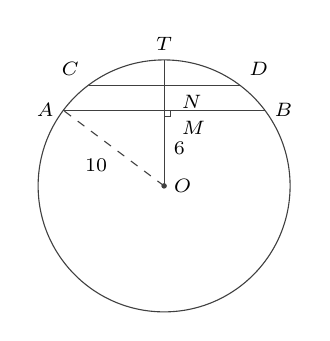
\begin{tikzpicture}[fig,every node/.style={font=\scriptsize}]
\coordinate (O) at (0,0); \coordinate (M) at (0,0.96); \coordinate (N) at (0,1.28); \coordinate (T) at (0,1.6); \coordinate (A) at (-1.28,0.96);
\draw (O) circle (1.6);
\draw (A) -- (1.28,0.96); \draw (-0.96,1.28) -- (0.96,1.28);
\draw (O) -- (T); \draw[dashed] (O) -- (A);
\draw (M) ++(0.08,0) -- ++(0,-0.08) -- ++(-0.08,0);
\fill[figline] (O) circle (0.035);
\node[right] at (O) {$O$}; \node[above] at (T) {$T$};
\node[left] at (A) {$A$}; \node[right] at (1.28,0.96) {$B$};
\node[above left] at (-0.96,1.28) {$C$}; \node[above right] at (0.96,1.28) {$D$};
\node[anchor=north west] at (0.1,0.95) {$M$}; \node[anchor=north west] at (0.1,1.27) {$N$};
\node[right] at (0,0.48) {$6$}; \node[below left] at (-0.6,0.46) {$10$};
\end{tikzpicture}
\end{minipage}
\end{answerblock}

\sect{Section E (case study, 4 marks)}

\Needspace{8\baselineskip}
\ques Case study. The sports ground of a school is a circle with centre $O$ and radius $29$~m. A flag post stands at $O$. For sports day, the PE teacher draws straight chalk lines from edge to edge of the ground as running tracks. Track $AB$ is $42$~m long.

\begin{center}
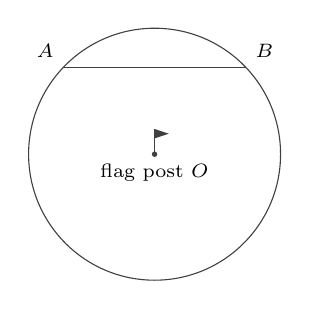
\begin{tikzpicture}[fig,every node/.style={font=\scriptsize}]
\coordinate (O) at (0,0);
\draw (O) circle (1.6);
\draw (-1.159,1.103) -- (1.159,1.103);
\fill[figline] (O) circle (0.035);
\draw (O) -- (0,0.32); \fill[figline] (0,0.32) -- (0.18,0.26) -- (0,0.2) -- cycle;
\node[below] at (O) {flag post $O$};
\node[above left] at (-1.159,1.103) {$A$}; \node[above right] at (1.159,1.103) {$B$};
\end{tikzpicture}
\end{center}

\pc{i}{Find the distance of track $AB$ from the flag post.\mks{1}}
\pc{ii}{Track $CD$ is also $42$~m long. Without calculating, write the distance of $CD$ from the flag post. Name the theorem you used.\mks{1}}
\pc{iii}{Compare $\angle AOB$ and $\angle COD$. Give the reason.\mks{1}}
\pc{iv}{Track $EF$ is $40$~m long. Is $EF$ nearer to the flag post or farther from it than $AB$? Find its distance from the flag post.\mks{1}}

\begin{answerblock}
\begin{minipage}[t]{0.66\linewidth}\vspace{0pt}
\Given radius $29$~m; $AB=CD=42$~m; $EF=40$~m.

\textbf{(i)} $AM=21$~m (Theorem 4); $OM^2=29^2-21^2=841-441=400$, so $OM=20$~m.

\textbf{(ii)} $20$~m: equal chords are equidistant from the centre (Theorem 6).

\textbf{(iii)} $\angle AOB=\angle COD$: equal chords subtend equal angles at the centre (Theorem 1).

\textbf{(iv)} $EF<AB$, so $EF$ is farther (Theorem 8). Half of $EF$ is $20$~m; $d^2=841-400=441$, so $d=21$~m.

\Ans (i) $20$~m; (ii) $20$~m; (iii) equal; (iv) farther, $21$~m.
\end{minipage}\hfill
\begin{minipage}[t]{0.3\linewidth}\vspace{0pt}
\centering
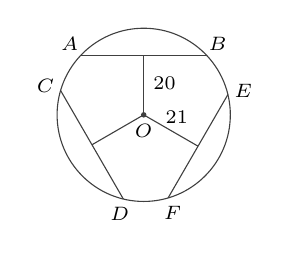
\begin{tikzpicture}[fig,every node/.style={font=\scriptsize}]
\coordinate (O) at (0,0);
\draw (O) circle (1.1);
\draw (-0.797,0.759) -- (0.797,0.759); \draw (-1.056,0.31) -- (-0.258,-1.07); \draw (1.07,0.259) -- (0.31,-1.055);
\draw (O) -- (0,0.759); \draw (O) -- (-0.657,-0.38); \draw (O) -- (0.69,-0.398);
\fill[figline] (O) circle (0.035);
\node[below] at (O) {$O$};
\node at (136.4:1.3) {$A$}; \node at (43.6:1.3) {$B$}; \node at (163.6:1.3) {$C$};
\node at (256.4:1.3) {$D$}; \node at (13.6:1.3) {$E$}; \node at (-73.6:1.3) {$F$};
\node[right] at (0,0.4) {$20$}; \node[above] at (0.42,-0.24) {$21$};
\end{tikzpicture}
\end{minipage}
\end{answerblock}
\end{document}
